\documentclass[tikz]{standalone}
\usepackage{tikz} 
\usetikzlibrary{shapes.misc,patterns,hobby}
\usepackage{pgfplots}
\usepgfplotslibrary{fillbetween}
%\usepackage[active,tightpage]{preview}  %generates a tightly fitting border around the work
%\PreviewEnvironment{tikzpicture}
%\setlength\PreviewBorder{2mm}
\usepackage{xcolor}
\definecolor{myred}{RGB}{196,19,47} 
\definecolor{myblue}{RGB}{0,139,139}

\begin{document}
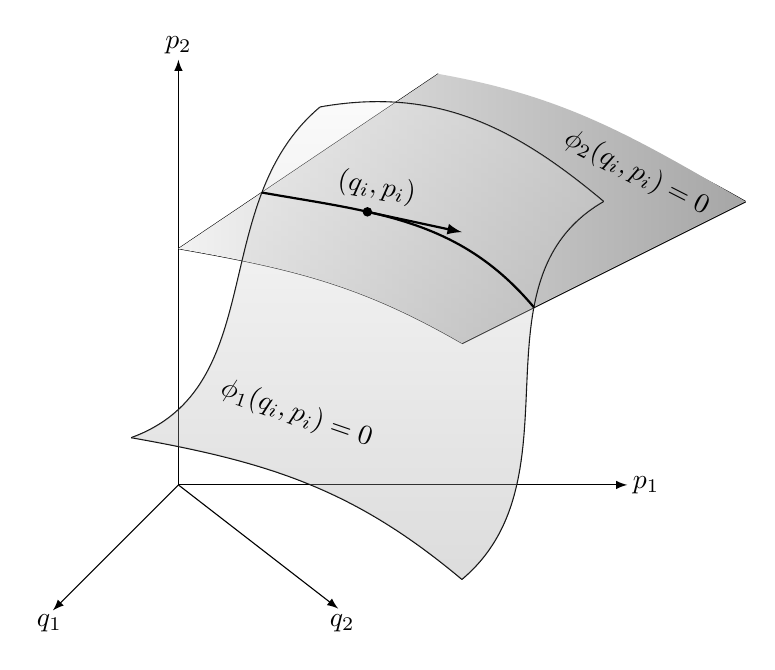
\begin{tikzpicture}[xscale=0.6,yscale=0.6,>=latex]

%Koordinatensystem (3D)
\draw[->, thin] (0,-5,0) to (0,-5,6.9);
\node at (0,-5.2,7.1) {$q_1$};
\draw[->, thin] (0,-5,0) to (6,-5,6.8);
\node at (6.2,-5.2,7.1) {$q_2$};
\draw[->, thin] (0,-5,0) to (9.5,-5,0);
\node at (9.9,-5,0) {$p_1$};
\draw[->, thin] (0,-5,0) to (0,4,0);
\node at (0,4.3,0) {$p_2$};


% This code is mainly from https://tex.stackexchange.com/questions/158585/draw-3d-intersecting-surfaces?rq=1

% border of the surface1
\path[draw,name path=border1] (0,0) to[out=-10,in=150] (6,-2);
% border of the surface1
\path[draw,name path=border2] (12,1) to[out=150,in=-10] (5.5,3.2);
% border of the surface1
\draw[draw,thick,name path=line1] (6,-2) -- (12,1);
% border of the surface1
\path[draw,name path=line2] (5.5,3.7) -- (0,0);
% draw the surface1
\shade[left color=gray!10,right color=gray!70] 
  (0,0) to[out=-10,in=150] (6,-2) -- 
  (12,1) to[out=150,in=-10] (5.5,3.7) -- cycle;

% border of the surface2
\path[draw,name path=border3] (-1,-4) to[out=20,in=220] (3,3);
% border of the surface2
\path[draw,name path=border4] (6,-7) to[out=40,in=210] (9,1);
% border of the surface2
\path[draw,name path=border5] (-1,-4) to[out=-10,in=140] (6,-7);
% border of the surface2
\path[draw,name path=border6] (3,3) to[out=10,in=140] (9,1);

% draw the surface2
\shade[top color=gray!10,bottom color=gray!90,opacity=.30] 
  (-1,-4) to[out=20,in=220] (3,3)  to[out=10,in=140] (9,1)
 to[out=210,in=40] (6,-7) to[out=140,in=-10] (-1,-4);

% intersection points
\path[name intersections={of=border3 and line2,by={a}}];
\path[name intersections={of=border4 and line1,by={b}}];

% intersection of the surfaces
\draw[thick] (a) to[out=-10,in=130] (b);

% labels
\node[rotate=-19] at (2.5,-3.5) {$\phi_1(q_i,p_i) = 0$};
\node[rotate=-27] at (9.7,1.6) {$\phi_2(q_i,p_i) = 0$};

% vector
\draw[->, thick] (4,0.78) to (6,0.35);
\node[rotate=-10] at (4.2,1.3) {$(q_i,p_i)$};
\filldraw (4,0.78) circle (2.5pt);

\end{tikzpicture}
\end{document}